\documentclass[conference]{assets/latex/IEEEtran}
\usepackage{amsmath,amssymb}
\usepackage{graphicx}
\graphicspath{{assets/latex/}}
\begin{document}
\title{CS6524 Computer Vision Lab 4\\Optical Flow and Kalman Filters}
\author{\IEEEauthorblockN{Ellice Nelson}
\IEEEauthorblockA{Student ID 23371323\\Immersive Software Engineering\\University of Limerick}}
\maketitle
\section{Methodology}
\subsection{Optical flow}
The program reads every MP4 in \texttt{in/} and saves optical-flow and tracking videos, plus CSV files of measurements and filter states.

We detect corners across the first frame and every five frames afterwards. Settings are 300 corners, quality level 0.01, minimum distance 8 pixels, and block size 7. Extra corners are added in moving areas every frame, using 200 corners, quality level 0.001, and minimum distance 6 pixels. To find these areas, we blur two frames with a $5\times5$ Gaussian filter, subtract them, keep differences above 15, and expand the mask with a $15\times15$ dilation. This gives smooth objects more chances to get features when the background has stronger corners.

Lucas--Kanade uses a $21\times21$ window and \texttt{maxLevel=3}. It stops after 30 iterations or an update below 0.01. We also track points backwards and reject those with a return error of at least 1 pixel. Points must move at least 1 pixel/frame to supply measurements. Static points are removed after 50 frames.

Points are grouped by similar velocity. Differences must be within 30\% of the reference speed, with a minimum allowance of 1 pixel/frame. We remove spatial outliers using three scaled median absolute deviations. Each group needs at least five points.

The mean position and mean velocity of a group form its measurement. We track this feature centre. Its position within the object can change when features are lost or added.

\subsection{Kalman filter}
We wrote the filter in NumPy. Its state is $[x,y,v_x,v_y]$, in pixels and pixels/frame. Prediction adds velocity to position each frame,
\begin{equation}
F=\begin{bmatrix}
1&0&1&0\\0&1&0&1\\0&0&1&0\\0&0&0&1
\end{bmatrix}.
\end{equation}
The measurement matrix uses all four measured values directly,
\begin{equation}
H=\begin{bmatrix}
1&0&0&0\\0&1&0&0\\0&0&1&0\\0&0&0&1
\end{bmatrix}.
\end{equation}
There is no control input.

The first measurement sets the initial state. The spread of feature positions and velocities sets the initial uncertainty $P$ and measurement noise $R$. Standard deviations have lower limits of 2 pixels and 0.3 pixels/frame. These values are squared to make variances.

Position noise also uses the median spread of the last 25 accepted measurements as a lower limit. This reduces trust in a tight group on a partly hidden object. Feature spread includes object size, so it is only an approximate measure of error.

Process noise $Q$ allows changes in velocity. We set acceleration standard deviation to 2 pixels/frame$^2$. With a one-frame step,
\begin{equation}
Q=\begin{bmatrix}
1&0&2&0\\0&1&0&2\\2&0&4&0\\0&2&0&4
\end{bmatrix}.
\end{equation}
The filter calculates the gain $K$ during corrections. Its diagonal values appear in the video. We use the Joseph covariance update to reduce rounding errors.

\subsection{Gaps and returning objects}
The tracker compares each group's position and velocity with the prediction using a distance test that accounts for uncertainty. The normal threshold is 18.47. New tracks need three matches and may miss up to two frames in a row.

When no suitable measurement is found, the filter keeps predicting. After at least five missed frames, a returning group needs three matches and must pass a second test, with threshold 23.51, against the saved prediction.

A copy of the earlier filter then continues without updates. The main path follows the returning measurements. The independent path stops extending when it leaves the image.

Measurements are white, corrections green, predictions orange, and independent paths magenta. Red lines connect predicted and measured return positions. Velocity arrows appear every five frames at four times their actual size. Ellipses show position uncertainty.

\section{Results, Discussion and Failure Analysis}
\begin{table}[t]
\centering
\caption{First recorded return. Frame numbering starts at zero.}
\label{tab:results}
\begin{tabular}{lrrr}
\hline
Object & Return frame & Gap (frames) & Error (px)\\
\hline
Orange & 59 & 22 & 208.1\\
Pen & 133 & 72 & 251.4\\
Potato & 86 & 14 & 95.4\\
Football & 61 & 13 & 161.1\\
\hline
\end{tabular}
\end{table}

Table~\ref{tab:results} uses the first recorded return after a gap of at least five frames. Error is the distance between the prediction and the returning optical-flow position, before correction. Values come from the CSVs. They measure agreement with the feature centre. We had no labelled object centres to measure true position error.

The orange returns after 22 frames with a 208.1-pixel error. Tracking resumes, but the path later moves across different parts of the orange as the feature group changes. This makes its tracked centre unstable.

The pen has the longest first gap, 72 frames, and the largest error, 251.4 pixels. Its uncertainty grows visibly while hidden. It loses measurements again later. Our speed cutoff can reject slow or stationary features even when the object is visible.

The potato has the smallest first return error, 95.4 pixels after 14 frames. Figure~\ref{fig:potato} shows the corrected path responding to new measurements while the independent path continues across the image. Changing visible features still shift the tracked centre.

\begin{figure}[t]
\centering
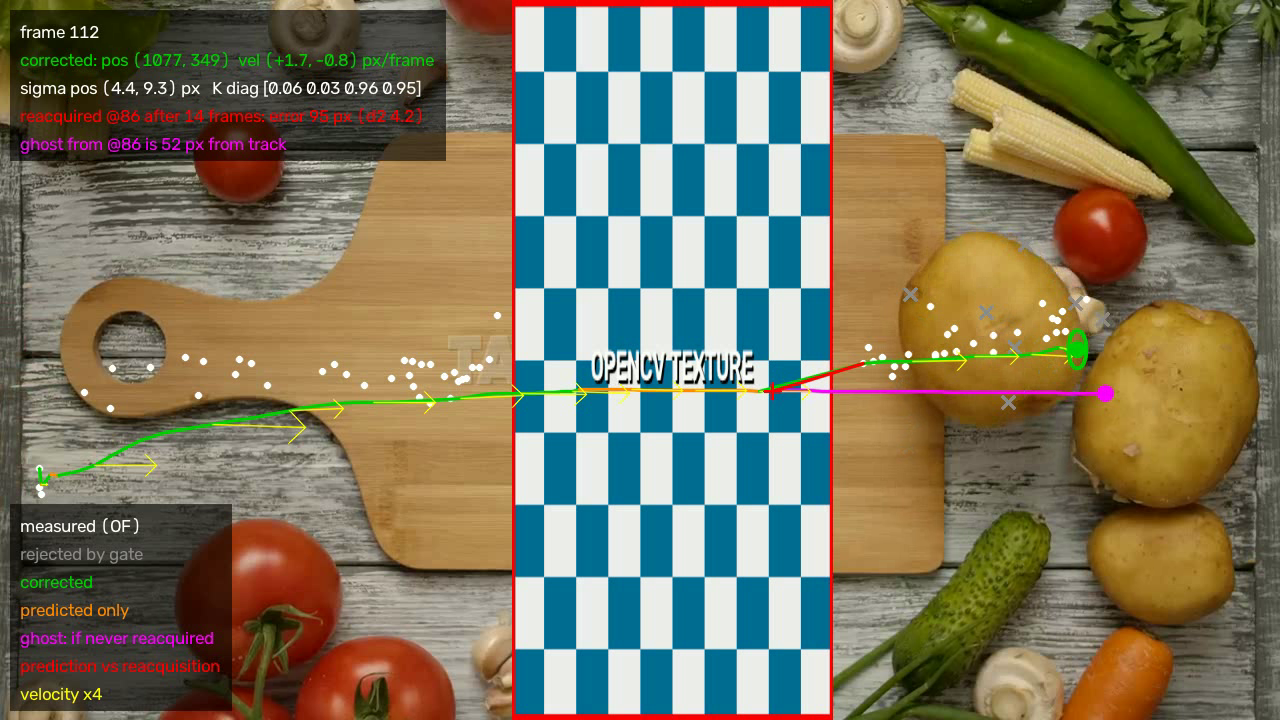
\includegraphics[width=\columnwidth]{potato.png}
\caption{Potato at frame 112. Green uses returning measurements. Magenta continues without corrections.}
\label{fig:potato}
\end{figure}

The extra video shows a football rolling behind a wooden obstruction. It returns after 13 missed frames with a 161.1-pixel error. Figure~\ref{fig:football} shows both paths after its return. Ball rotation and the person's hand create changing or competing features.

\begin{figure}[t]
\centering
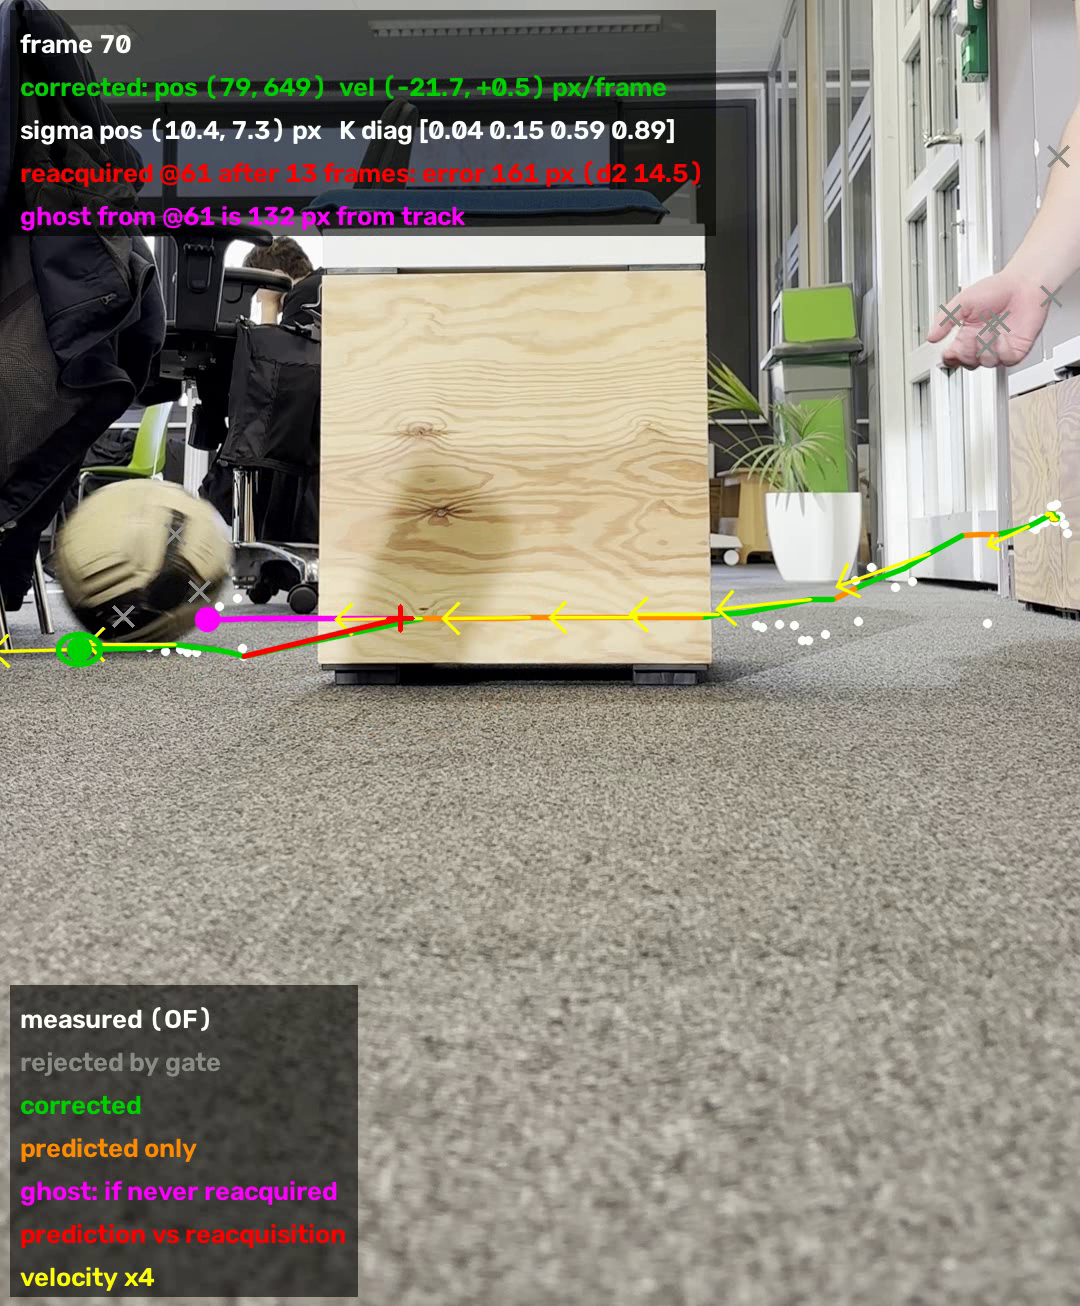
\includegraphics[width=\columnwidth,height=0.25\textheight,keepaspectratio]{football.png}
\caption{Football at frame 70. Red marks the return error. Magenta keeps the earlier motion estimate.}
\label{fig:football}
\end{figure}

\subsection{Failures and improvements}
The orange CSV contains backward frame steps, including $90\rightarrow86$. Selecting a new track can add saved records that overlap earlier ones. This also affects agreement between final records and frames already drawn. We avoided tracking percentages based on row counts. We would fix this by keeping one main-track record per frame and drawing the video after tracking finishes.

To reduce centre shifts, we would keep feature offsets from a fixed object reference when adding points. Matching appearance would help separate the object from hands and other moving objects. Allowing reliable updates when the object stops would reduce gaps caused by the speed cutoff. Manually marking reference positions would let us measure true error and tune the noise values against those measurements.
\end{document}
